\chapter{Lực, không gian pha và các định luật bảo toàn}

\lectureoverview{Một định luật chuyển động phải làm nhiều hơn việc liên hệ các đại lượng vật lý quen thuộc. Nó phải xác định trạng thái của một hệ, đưa trạng thái ấy từ thời điểm này sang thời điểm tiếp theo, và cho thấy những phân biệt và đại lượng nào còn được bảo toàn qua chuyển động. Ta sẽ đi tới cơ học Newton bằng cách trước hết kiểm tra một định luật lực có vẻ hợp lý nhưng sai, rồi mở rộng trạng thái từ vị trí sang không gian pha, và cuối cùng suy ra sự bảo toàn động lượng và năng lượng.}

\section{Một định luật sai nhưng hữu ích}

Chuyển động thường ngày bị ma sát chi phối. Hãy đẩy một vật nặng trên sàn thì nó chuyển động; ngừng đẩy và nó sớm dừng lại. Một lực đẩy lớn hơn nói chung tạo ra tốc độ lớn hơn, còn một vật nặng hơn thì đòi hỏi phải đẩy mạnh hơn. Trong một thế giới như vậy, thật tự nhiên khi cho rằng lực trực tiếp tạo ra vận tốc. Đó là trực giác cơ bản đứng sau mô tả chuyển động kiểu Aristotle.

Trượt băng đem lại trải nghiệm còn thiếu. Một người trượt băng cần lực để bắt đầu, dừng lại hoặc đổi hướng, nhưng không cần lực để tiếp tục lướt một khi đã chuyển động. Nếu Aristotle làm việc trên mặt băng gần như không ma sát thay vì trên mặt đất thông thường, thì khiếm khuyết của trực giác lực--vận tốc hẳn đã khó bị bỏ sót hơn nhiều.

Để phơi bày chỗ sai của trực giác ấy, ta hãy cho nó một dạng hiện đại chính xác. Ta viết phương trình cố ý sai sau đây

\begin{equation}
  \mathbf F=m\mathbf v.
  \label{eq:aristotle-vector-law}
\end{equation}

Đây không phải là định luật Newton và không nên học thuộc như một mệnh đề vật lý. Giá trị của nó có tính chẩn đoán: một khi một quy tắc bằng lời đã trở thành một phương trình, ta có thể hỏi liệu nó có dự đoán được chuyển động hay không và liệu nó có giữ lại đủ thông tin để tái dựng quá khứ hay không. Cuộc thảo luận ngắn trên lớp về từ Hy Lạp chỉ lực dẫn đến \emph{dynamis}, gốc từ cũng nghe thấy trong những từ như dynamo và dynamics, nhưng thuật ngữ là thứ yếu so với việc kiểm nghiệm chính định luật ấy.

\begin{figure}[htbp]
  \centering
  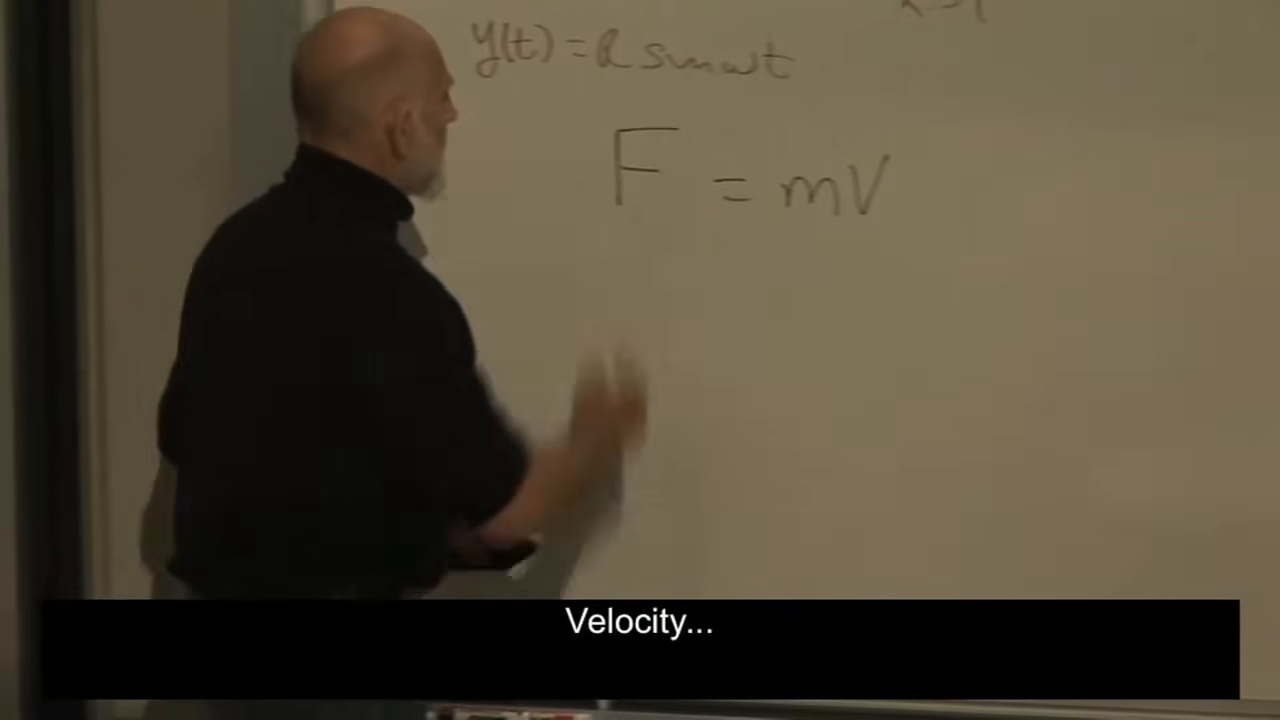
\includegraphics[width=0.82\textwidth]{lecture_02_figure_02.png}
  \caption{Định luật lực--vận tốc cố ý sai, được dùng để kiểm tra tính dự đoán và tính thuận nghịch.}
  \lectureframe{00:04:51}
\end{figure}

Giới hạn chuyển động vào một tọa độ không gian. Vì \(v=\dot x\), định luật có dạng

\begin{equation}
  F(t)=m\dot x(t).
  \label{eq:aristotle-1d}
\end{equation}

Bây giờ chia thời gian thành các khoảng ngắn có độ dài \(\delta\). Trong một khoảng,

\begin{equation}
  \dot x(t)\simeq
  \frac{x(t+\delta)-x(t)}{\delta}.
  \label{eq:first-difference}
\end{equation}

Thế vào phương trình~\eqref{eq:aristotle-1d} ta được

\begin{equation}
  x(t+\delta)
  =x(t)+\frac{\delta}{m}F(t).
  \label{eq:aristotle-update}
\end{equation}

Điều này mang dạng của một quy tắc cập nhật thực sự. Nếu biết vị trí hiện tại và lực, thì vị trí ở thời điểm lấy mẫu kế tiếp được xác định. Tuy nhiên, khi lực triệt tiêu, quy tắc của Aristotle cho \(\dot x=0\): vật phải đứng yên. Chuyển động không có lực duy trì bị loại bỏ ngay từ đầu.

\begin{figure}[htbp]
  \centering
  \includegraphics[width=0.84\textwidth]{lecture_02_figure_07.png}
  \caption{Quy tắc cập nhật rời rạc kiểu Aristotle với một lực phục hồi. Mỗi bước nhân độ dời với một hệ số nhỏ hơn 1 một chút.}
  \lectureframe{00:10:15}
\end{figure}

\subsection{Lò xo trong cơ học Aristotle}

Xét một hạt gắn với một lò xo, có vị trí cân bằng tại \(x=0\). Một độ dời sinh ra lực phục hồi

\begin{equation}
  F(x)=-kx,
  \qquad k>0.
  \label{eq:hooke-law}
\end{equation}

Thay lực này vào phương trình~\eqref{eq:aristotle-update} cho

\begin{equation}
  x(t+\delta)
  =\left(1-\frac{k\delta}{m}\right)x(t).
  \label{eq:aristotle-spring-update}
\end{equation}

Với \(\delta\) đủ nhỏ, thừa số trong ngoặc chỉ hơi nhỏ hơn 1. Vì thế, mỗi lần cập nhật đều làm giảm độ dời đi cùng một tỉ phần:

\begin{equation}
  x_n=\left(1-\frac{k\delta}{m}\right)^n x_0.
  \label{eq:aristotle-geometric-decay}
\end{equation}

Phương trình liên tục và nghiệm của nó là

\begin{align}
  m\dot x&=-kx,
  \label{eq:aristotle-spring-continuous}\\
  x(t)&=x(0)e^{-kt/m}.
  \label{eq:aristotle-spring-solution}
\end{align}

Lò xo không dao động. Khi được thả từ bất kỳ độ dời nào, nó tiến về gốc theo hàm mũ, chuyển động ngày càng chậm khi tiến lại gần.

\begin{figure}[htbp]
  \centering
  \includegraphics[width=0.84\textwidth]{lecture_02_figure_08.png}
  \caption{Nghiệm hàm mũ của phương trình lò xo kiểu Aristotle. Độ dời suy giảm chứ không dao động.}
  \lectureframe{00:12:02}
\end{figure}

Tương lai thì dễ dự đoán: mọi độ dời ban đầu đều tiến đến cùng một cấu hình nghỉ. Quá khứ lại là chuyện khác. Giả sử hạt được quan sát ở rất gần gốc tọa độ nhưng chỉ với độ chính xác hữu hạn. Nó có thể đã bắt đầu từ bất kỳ độ dời nào trong nhiều độ dời khác nhau, vì những phần còn lại nhỏ theo hàm mũ của tất cả chúng cuối cùng đều nằm trong cùng một dung sai đo. Với độ chính xác toán học hoàn hảo, phương trình~\eqref{eq:aristotle-spring-solution} có thể được chạy ngược, nhưng những khác biệt thực tế giữa các lịch sử thì liên tục bị xóa mờ. Vì thế, xét từ quan điểm của động lực học cơ bản có tính thuận nghịch, định luật này là đáng ngờ.

Điều này không có nghĩa Aristotle là phi lý. Kiểu chuyển động bị ma sát chi phối mà ông mô tả thực sự là tiêu tán. Sai lầm là nâng hành vi hiệu dụng đó lên thành một định luật cơ bản. Bản thân ma sát cũng là một lực nảy sinh từ những tương tác vi mô phức tạp. Khi một bàn tay đẩy một vật với tốc độ xấp xỉ không đổi, lực tác dụng đang cân bằng ma sát; lực tác dụng không phải tự thân đang tạo ra vận tốc.

\section{Định luật Newton và ý nghĩa vật lý của nó}

Hiệu chỉnh theo Newton là: lực làm thay đổi chuyển động:

\begin{equation}
  \mathbf F=m\mathbf a=m\ddot{\mathbf x}.
  \label{eq:newton-second-law}
\end{equation}

Trước khi xem đây như một phương trình tiến hóa, phải gỡ ra hai chỗ có vẻ vòng tròn. Chỗ thứ nhất liên quan đến hệ quy chiếu. Người ta thường nghe nói rằng các định luật Newton đúng trong các hệ quy chiếu quán tính và rằng hệ quy chiếu quán tính là hệ trong đó các định luật Newton đúng. Khẳng định vật lý không phải là định nghĩa vòng tròn đó. Nó là mệnh đề thực nghiệm rằng có \emph{tồn tại} những hệ quy chiếu, được mô tả bởi các thước và đồng hồ thích hợp, trong đó các định luật Newton có dạng đơn giản. Những hệ quy chiếu đang gia tốc hoặc quay so với chúng đòi hỏi thêm các lực biểu kiến. Cách các phương trình biến đổi trong những hệ khác ấy có thể được khảo sát sau.

Chỗ vòng tròn thứ hai liên quan đến lực và khối lượng. Nếu lực được định nghĩa là khối lượng nhân gia tốc, còn khối lượng là lực chia cho gia tốc, thì phương trình dường như rỗng nội dung. Một thí nghiệm thao tác tách các định nghĩa ra khỏi định luật. Hãy so sánh một vật với một kilôgam chuẩn bằng cách cân bằng hai bên, rồi gắn vật đó vào một lực kế lò xo trong một không gian ngoài ra không có lực. Định nghĩa một đơn vị lực bằng một độ dãn nhỏ cố định của lò xo. Hai lò xo giống hệt nhau, mỗi lò xo bị kéo dãn đúng bằng lượng ấy, cho hai đơn vị lực và tạo ra gia tốc gấp đôi. Thêm lò xo thứ hai an toàn hơn là kéo một lò xo đi xa gấp đôi, vì một lò xo thực cuối cùng sẽ trở nên phi tuyến hoặc bị gãy. Vẫn dùng một lò xo nhưng ghép thêm hai khối lượng bằng nhau thì gia tốc bằng một nửa; ba khối lượng bằng nhau thì bằng một phần ba.

\begin{figure}[htbp]
  \centering
  \includegraphics[width=0.84\textwidth]{lecture_02_figure_09.png}
  \caption{Thí nghiệm tưởng tượng với lực kế lò xo dùng để định nghĩa các đơn vị lực bằng nhau và kiểm tra việc gia tốc tỉ lệ với lực.}
  \lectureframe{00:22:45}
\end{figure}

Những phép so sánh này đem lại nội dung thực nghiệm cho

\begin{equation}
  a\propto F,
  \qquad
  a\propto\frac{1}{m},
  \qquad
  F=ma.
  \label{eq:force-mass-scaling}
\end{equation}

Từ \emph{particle} sẽ được dùng cho mọi vật nhỏ mà cấu trúc bên trong không liên quan, chứ không chỉ cho một hạt sơ cấp.

\subsection{Vì sao chỉ vị trí thôi chưa phải là trạng thái}

Giờ ta kiểm tra phương trình Newton bằng cùng phương pháp stroboscopic. Sai phân hữu hạn đối xứng cho gia tốc là

\begin{equation}
  \ddot x(t)\simeq
  \frac{x(t+\delta)-2x(t)+x(t-\delta)}{\delta^2}.
  \label{eq:second-difference}
\end{equation}

Do đó phương trình Newton kéo theo

\begin{equation}
  x(t+\delta)
  =2x(t)-x(t-\delta)+\frac{\delta^2}{m}F(t).
  \label{eq:newton-position-update}
\end{equation}

Vị trí kế tiếp không thể thu được chỉ từ \(x(t)\). Ta còn cần vị trí trước đó \(x(t-\delta)\), hay tương đương là vận tốc ở thời điểm hiện tại. Lúc đầu điều này khiến phương trình Newton có vẻ kém khả năng dự đoán hơn phương trình của Aristotle. Kết luận đúng, trái lại, là chỉ riêng vị trí vốn là một mô tả không đầy đủ của trạng thái. Biết mọi thứ liên quan tại một thời điểm có nghĩa là biết đủ dữ liệu để xác định chuyển động tiếp theo. Đối với một hạt Newton, các dữ liệu đó là vị trí và vận tốc.

\section{Động lượng và không gian pha}

Định nghĩa động lượng bởi

\begin{equation}
  \mathbf p=m\mathbf v=m\dot{\mathbf x}.
  \label{eq:momentum-definition}
\end{equation}

Khối lượng của một hệ Newton cố định được xem là không đổi. Một vật có thể mất đi một phần, như cây bút có thể mất nắp, nhưng khi đó vật đang được mô tả đã thay đổi; hệ kín được chọn vẫn có tổng khối lượng không đổi. Với \(m\) không đổi, định luật thứ hai của Newton trở thành

\begin{equation}
  \mathbf F=\dot{\mathbf p}.
  \label{eq:newton-momentum-form}
\end{equation}

\begin{figure}[htbp]
  \centering
  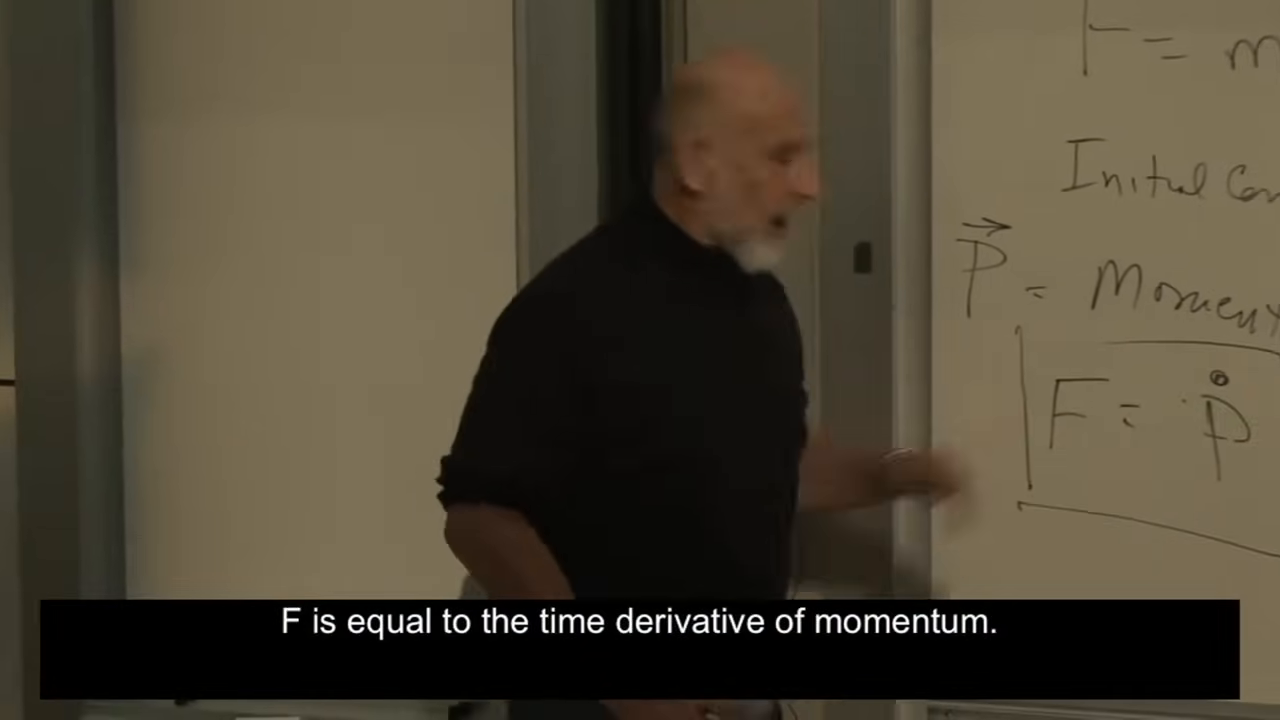
\includegraphics[width=0.82\textwidth]{lecture_02_figure_03.png}
  \caption{Định luật Newton được viết dưới dạng đạo hàm theo thời gian của động lượng.}
  \lectureframe{00:32:35}
\end{figure}

Đối với một tọa độ, chuyển động Newton giờ có thể được viết thành 2 phương trình bậc nhất cho 2 biến trạng thái độc lập:

\begin{align}
  \dot p&=F(x,t),
  \label{eq:first-order-p}\\
  \dot x&=\frac{p}{m}.
  \label{eq:first-order-x}
\end{align}

Một phương trình cho biết lực làm đổi động lượng như thế nào; phương trình kia cho biết động lượng làm đổi vị trí như thế nào. Dạng rời rạc bậc nhất của chúng là

\begin{align}
  p(t+\delta)&=p(t)+\delta F(x(t),t)+O(\delta^2),
  \label{eq:momentum-discrete}\\
  x(t+\delta)&=x(t)+\frac{\delta}{m}p(t)+O(\delta^2).
  \label{eq:position-discrete}
\end{align}

Biết \(x(t)\) và \(p(t)\), các phương trình này xác định cặp kế tiếp; cặp ấy rồi trở thành dữ liệu đầu vào cho bước sau. Quỹ đạo được dựng lên bằng các lần cập nhật lặp lại.

\begin{figure}[htbp]
  \centering
  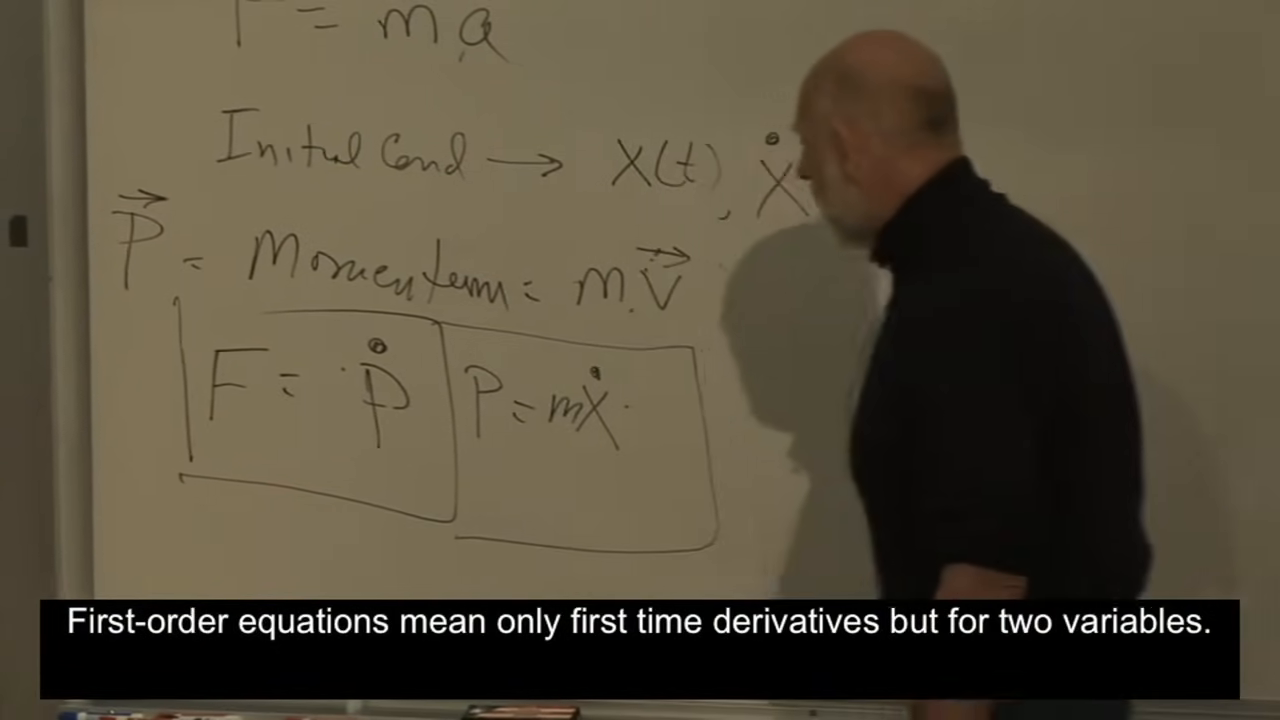
\includegraphics[width=0.84\textwidth]{lecture_02_figure_04.png}
  \caption{Hai phương trình bậc nhất và dữ liệu đầu tương ứng. Vị trí và động lượng cùng nhau xác định trạng thái.}
  \lectureframe{00:35:47}
\end{figure}

Không gian của mọi cặp \((x,p)\) được gọi là \emph{không gian pha}. Với 1 hạt chuyển động trong 3 chiều, nó có 6 tọa độ,

\begin{equation}
  (x,y,z,p_x,p_y,p_z).
  \label{eq:one-particle-phase-space}
\end{equation}

Không gian pha là không gian của các điều kiện đầu đầy đủ. Không gian cấu hình chỉ ghi các vị trí; không gian pha ghi đúng những dữ liệu mà định luật chuyển động cần đến.

\begin{classroomqa}
  \audiencequestion{Nếu lực là một hàm của vị trí chứ không phải một hàm đã biết của thời gian, thì việc cập nhật có trở nên phức tạp hơn không?\lecturetimestamp{00:36:27--00:37:07}}
  \lecturerresponse{Các phương trình vẫn có tính dự đoán. Một khi đã biết \(x\) và \(p\), thì giá trị \(F(x)\) được biết. Phương trình~\eqref{eq:first-order-p} cập nhật \(p\), phương trình~\eqref{eq:first-order-x} cập nhật \(x\), và cặp đã cập nhật lại có thể được dùng tiếp.}
\end{classroomqa}

\section{Lò xo Newton}

Hãy quay lại lò xo để có thể so sánh hai định luật trên cùng một cơ sở vật lý. Newton cho

\begin{equation}
  m\ddot x=-kx.
  \label{eq:newton-spring}
\end{equation}

Tạm đặt \(m=k=1\) để loại bỏ các hằng số. Khi đó

\begin{equation}
  \ddot x=-x.
  \label{eq:normalized-oscillator}
\end{equation}

Không giống hàm mũ, hàm sin hay cos sau hai lần lấy đạo hàm thì trở về âm của chính nó. Nghiệm tổng quát có thể viết

\begin{align}
  x(t)&=C\cos(t-t_0),
  \label{eq:oscillator-x}\\
  p(t)=\dot x(t)&=-C\sin(t-t_0).
  \label{eq:oscillator-p}
\end{align}

Hai hằng số mang hai mẩu thông tin ban đầu. Biên độ \(C\) cho độ dời cực đại, còn \(t_0\) ấn định pha, được chọn ở đây sao cho vận tốc bằng không tại \(t=t_0\). Hạt chỉ dừng lại trong chốc lát ở hai đầu mút. Sau đó nó quay lại đi qua gốc, nơi tốc độ và động lượng của nó là lớn nhất, rồi tiếp tục dao động.

Bình phương các phương trình~\eqref{eq:oscillator-x} và \eqref{eq:oscillator-p} ta được

\begin{equation}
  x^2+p^2=C^2.
  \label{eq:oscillator-phase-circle}
\end{equation}

Vì vậy, điểm trong không gian pha chuyển động trên một đường tròn bán kính \(C\). Những biên độ ban đầu khác nhau cho những đường tròn khác nhau; thay đổi \(t_0\) chọn một điểm xuất phát khác trên cùng đường tròn. Trong các đơn vị đã chuẩn hóa này, mọi đường tròn đều được đi hết với cùng chu kỳ \(2\pi\), không phụ thuộc biên độ.

\begin{figure}[htbp]
  \centering
  \includegraphics[width=0.84\textwidth]{lecture_02_figure_10.png}
  \caption{Nghiệm của bộ dao động và quỹ đạo tròn của nó trong mặt phẳng pha \((x,p)\).}
  \lectureframe{00:43:20}
\end{figure}

\begin{figure}[htbp]
  \centering
  \begin{tikzpicture}[scale=1.05,>=Latex]
    \draw[->] (-2.6,0) -- (2.75,0) node[right] {$x$};
    \draw[->] (0,-2.4) -- (0,2.55) node[above] {$p$};
    \draw[blue!65!black,thick] (0,0) circle (1.85);
    \draw[->,blue!65!black,thick]
      (1.60,0.93) arc[start angle=30,end angle=72,radius=1.85];
    \fill[red!65!black] (1.60,0.93) circle (2pt);
    \draw[dashed] (0,0) -- (1.60,0.93)
      node[midway,below right] {$C$};
    \node[align=left] at (-1.55,1.85)
      {$x=C\cos(t-t_0)$\\$p=-C\sin(t-t_0)$};
  \end{tikzpicture}
  \caption{Một quỹ đạo trong không gian pha giữ lại cả vị trí lẫn động lượng. Bán kính của nó gắn nhãn cho chuyển động, còn góc thì tăng đều theo thời gian.}
  \label{fig:oscillator-phase-space}
\end{figure}

Phép chiếu lên trục ngang cho chuyển động qua lại quen thuộc của \(x\); phép chiếu lên trục đứng cho dao động của \(p\). Khác với lò xo kiểu Aristotle, các đường tròn khác nhau không bao giờ nhập vào nhau. Biết một điểm trong không gian pha quyết định cả tương lai lẫn quá khứ của nó.

Với \(m\) và \(k\) tổng quát, tần số góc là

\begin{equation}
  \omega=\sqrt{\frac{k}{m}},
  \qquad
  x(t)=C\cos\bigl(\omega(t-t_0)\bigr),
  \label{eq:general-oscillator-frequency}
\end{equation}

và quỹ đạo trong không gian pha trở thành một elip trong mặt phẳng \((x,p)\) chưa được chuẩn hóa. Bức tranh hình tròn là cách chuẩn hóa tiện lợi \(m=k=1\) được dùng trong bài giảng.

\begin{classroomqa}
  \audiencequestion{Nếu đạo hàm bậc hai trong phương trình bộ dao động được thay bằng đạo hàm bậc nhất, thì tính dự đoán có mất đi không?\lecturetimestamp{00:45:23--00:46:04}}
  \lecturerresponse{Không. Một phương trình bậc nhất vẫn có thể dự đoán chuyển động về phía trước từ dữ liệu đầu thích hợp. Vấn đề mạnh hơn là liệu dòng tiến hóa của nó có bảo toàn các phân biệt đủ tốt để có thể thuận nghịch hay không; định lý tổng quát liên quan được để lại đến khi có đủ công cụ cần thiết.}
\end{classroomqa}

\section{Đảo ngược thời gian}

Bức tranh bộ dao động làm cho tính thuận nghịch trở nên cụ thể, nhưng cũng có một phép kiểm tra trực tiếp trên các phương trình. Hãy đưa vào một tọa độ thời gian đảo ngược

\begin{equation}
  T=-t.
  \label{eq:reverse-time}
\end{equation}

Khi đó

\begin{equation}
  \frac{d}{dt}=-\frac{d}{dT},
  \qquad
  \frac{d^2}{dt^2}=\frac{d^2}{dT^2}.
  \label{eq:time-derivative-parity}
\end{equation}

Đạo hàm bậc nhất đổi dấu dưới phép đảo ngược thời gian, còn đạo hàm bậc hai thì không. Do đó, phương trình Aristotle tự trị

\begin{equation}
  m\dot x=F(x)
  \label{eq:aristotle-time-reversal}
\end{equation}

không giữ nguyên dạng của nó khi một thước phim được chiếu ngược. Một lò xo đang suy giảm sẽ trở thành một lò xo tự phát rời khỏi cân bằng. Trái lại,

\begin{equation}
  m\ddot x=F(x)
  \label{eq:newton-time-reversal}
\end{equation}

vẫn không đổi. Khi chiếu ngược một đoạn phim Newton, vận tốc đổi dấu nhưng gia tốc thì không, nên đoạn phim chạy ngược lại là một nghiệm được phép khác.

\begin{figure}[htbp]
  \centering
  \includegraphics[width=0.84\textwidth]{lecture_02_figure_11.png}
  \caption{So sánh trên bảng dưới phép \(t\mapsto -t\): các đạo hàm bậc nhất đổi dấu, còn các đạo hàm bậc hai thì không.}
  \lectureframe{00:50:45}
\end{figure}

\begin{classroomqa}
  \audiencequestion{Vì sao nên chấp nhận tính đảo ngược như một tiền đề về vật lý nói chung?\lecturetimestamp{00:46:16--00:48:26}}
  \lecturerresponse{Đó là điều được kiểm nghiệm chứ không phải được bảo đảm bằng định nghĩa. Ta khảo sát các định luật thành công, nhận diện những đặc trưng thực nghiệm chung, rồi nâng chúng lên thành các nguyên lý. Trật tự lôgic sâu hơn lại theo chiều ngược lại: lý thuyết trường lượng tử là nền tảng hơn, còn cơ học Newton xuất hiện thông qua những gần đúng như chuyển động chậm và các vật nặng. Một khóa học phải xây dựng đi lên từ các định luật đơn giản hơn, nên bây giờ tính đảo ngược được đưa vào như một nguyên lý mà phạm vi hiệu lực của nó sẽ được kiểm nghiệm về sau.}
\end{classroomqa}

\begin{classroomqa}
  \audiencequestion{Bản thân tính đảo ngược có phải là một vấn đề mà Newton ý thức rõ hay không?\lecturetimestamp{00:48:28--00:49:02}}
  \lecturerresponse{Câu trả lời về mặt lịch sử là không chắc chắn. Chắc chắn Newton hiểu quán tính: lực là cần thiết để làm thay đổi trạng thái chuyển động, chứ không phải để duy trì chuyển động thẳng đều. Việc ông có phát biểu nhận xét đó một cách tường minh theo ngôn ngữ của tính đảo ngược hay không lại là một câu hỏi lịch sử khác.}
\end{classroomqa}

\section{Chu trình và các đại lượng bảo toàn}

Các đường tròn trong không gian pha gợi ra ý tưởng tiếp theo. Một quỹ đạo nằm trên một đường tròn và không bao giờ nhảy sang đường khác. Vì vậy, có thể gán cho mỗi đường tròn một con số không đổi dọc theo chuyển động. Với dao động tử đã chuẩn hóa, con số đó là

\begin{equation}
  C^2=x^2+p^2.
  \label{eq:cycle-label}
\end{equation}

Ngoại trừ một thừa số một nửa, đây là năng lượng của dao động tử. Đường tròn càng lớn thì năng lượng càng lớn; thay đổi pha ban đầu không làm nó thay đổi. Chúng ta sẽ suy ra mệnh đề ấy thay vì chỉ đọc nó từ hình vẽ, nhưng trước hết hãy xét động lượng.

Định luật thứ nhất của Newton nói rằng một vật không chịu hợp lực thì chuyển động với vận tốc không đổi. Điều ấy đã được bao hàm trong định luật thứ hai:

\begin{equation}
  \mathbf F=0
  \quad\Longrightarrow\quad
  \dot{\mathbf p}=0
  \quad\Longrightarrow\quad
  \mathbf v=\text{constant}
  \label{eq:newton-first-from-second}
\end{equation}

khi khối lượng không đổi. Định luật thứ ba của Newton thực sự cung cấp thông tin mới về các tương tác giữa các hạt.

\subsection{Các lực bằng nhau, ngược chiều và trung tâm}

Ký hiệu \(\mathbf F_{ij}\) là lực do hạt \(j\) tác dụng lên hạt \(i\). Phần bằng nhau và ngược chiều của định luật thứ ba là

\begin{equation}
  \mathbf F_{ij}=-\mathbf F_{ji}.
  \label{eq:newton-third-pair}
\end{equation}

Nếu hai lực cùng hướng, thì một cặp cô lập có thể tự phát gia tốc. Khi đó sẽ là một cỗ máy không cần chất đẩy mà chỉ từ các lực nội tại đã sinh ra chuyển động. Hành vi như vậy không được quan sát thấy.

\begin{figure}[htbp]
  \centering
  \includegraphics[width=0.84\textwidth]{lecture_02_figure_12.png}
  \caption{Phát biểu có chỉ số của các lực tương tác bằng nhau và ngược chiều.}
  \lectureframe{00:59:25}
\end{figure}

Đối với các lực giữa các hạt điểm được xét ở đây, cặp lực đó còn cùng tác dụng dọc theo đường nối tâm hai hạt. Các lực bằng nhau và ngược chiều nhưng không cùng phương có thể tạo thành một ngẫu lực thuần túy và làm một cặp vật rắn cô lập quay. Điều kiện lực trung tâm loại trừ khả năng đó:

\begin{equation}
  \mathbf F_{ij}\parallel
  (\mathbf r_i-\mathbf r_j).
  \label{eq:central-force-condition}
\end{equation}

Điều kiện bằng nhau và ngược chiều sẽ dẫn đến định luật bảo toàn động lượng tuyến tính. Điều kiện đường nối tâm gắn với bảo toàn mômen động lượng, điều sẽ được nghiên cứu sau.

\begin{figure}[htbp]
  \centering
  \includegraphics[width=0.84\textwidth]{lecture_02_figure_13.png}
  \caption{Phần lực trung tâm của định luật thứ ba Newton: các lực tương tác nằm dọc theo đường nối hai hạt.}
  \lectureframe{01:01:38}
\end{figure}

\subsection{Tổng động lượng}

Xét một hệ kín gồm \(N\) hạt. Không có lực ngoài; các lực duy nhất là những lực các hạt tác dụng lẫn nhau. Tính cộng của lực và định luật thứ hai Newton cho, đối với mỗi hạt,

\begin{equation}
  \dot{\mathbf p}_i
  =m_i\ddot{\mathbf r}_i
  =\sum_{\substack{j=1\\j\ne i}}^N \mathbf F_{ij}.
  \label{eq:many-particle-newton}
\end{equation}

Lấy tổng phương trình này theo \(i\):

\begin{align}
  \frac{d}{dt}\sum_{i=1}^N\mathbf p_i
  &=\sum_{i=1}^N
    \sum_{\substack{j=1\\j\ne i}}^N\mathbf F_{ij}
  \notag\\
  &=\sum_{i<j}\bigl(\mathbf F_{ij}+\mathbf F_{ji}\bigr)
  =0.
  \label{eq:momentum-pair-cancellation}
\end{align}

Mỗi tương tác xuất hiện hai lần, một lần theo mỗi chiều, và cả cặp triệt tiêu nhau. Định nghĩa

\begin{equation}
  \mathbf P_{\mathrm{tot}}=\sum_{i=1}^N\mathbf p_i,
  \label{eq:total-momentum}
\end{equation}

ta thu được định luật bảo toàn đầu tiên:

\begin{equation}
  \frac{d\mathbf P_{\mathrm{tot}}}{dt}=0.
  \label{eq:momentum-conservation}
\end{equation}

\begin{figure}[htbp]
  \centering
  \includegraphics[width=0.84\textwidth]{lecture_02_figure_14.png}
  \caption{Cộng các phương trình của các hạt làm các lực từng cặp triệt tiêu, để lại đạo hàm của tổng động lượng bằng không.}
  \lectureframe{01:04:38}
\end{figure}

Về mặt lịch sử, ta đã trình bày sự bảo toàn động lượng như một hệ quả của định luật thứ ba Newton. Vật lý hiện đại thường xem bảo toàn động lượng là phát biểu cơ bản hơn: nếu một hệ cô lập gồm hai hạt bảo toàn tổng động lượng, thì các độ biến thiên động lượng nội tại của nó phải bằng nhau và ngược chiều. Tuy nhiên, đối với tiến trình trình bày hiện tại, con đường Newton là con đường hữu ích.

\section{Năng lượng trong một chiều}

Xét một hạt chuyển động trên một đường thẳng dưới tác dụng của một lực chỉ phụ thuộc vào vị trí của nó:

\begin{equation}
  F=F(x).
  \label{eq:position-force}
\end{equation}

Một lực như vậy được gọi là không phụ thuộc thời gian. Điều đó không có nghĩa là lực mà hạt đang chuyển động cảm nhận có giá trị số không đổi. Giá trị của nó thay đổi khi \(x(t)\) thay đổi. Điều đó có nghĩa là mỗi khi hạt ở cùng một vị trí \(x\), nó chịu cùng một lực, bất kể thời điểm trên đồng hồ.

Trong một chiều, mọi hàm lực đủ trơn đều có thể lấy tích phân. Vì vậy ta định nghĩa thế năng \(V(x)\) bằng

\begin{equation}
  F(x)=-\frac{dV}{dx},
  \label{eq:potential-definition-1d}
\end{equation}

hay tương đương là

\begin{equation}
  V(x)=-\int^x F(u)\,du+V_0.
  \label{eq:potential-integral}
\end{equation}

Hằng số cộng \(V_0\) không ảnh hưởng đến lực. Hãy hình dung \(V(x)\) như độ cao của một địa hình phía trên trục \(x\). Hạt bị đẩy về phía độ cao thấp hơn, và lực lớn hơn ở nơi độ dốc lớn hơn. Ở đỉnh hoặc đáy của một ngọn đồi trơn, độ dốc triệt tiêu, nên lực cũng triệt tiêu tại đó.

\begin{figure}[htbp]
  \centering
  \includegraphics[width=0.84\textwidth]{lecture_02_figure_15.png}
  \caption{Thế năng như một địa hình một chiều. Lực hướng xuống dốc và có độ lớn do độ dốc quyết định.}
  \lectureframe{01:12:57}
\end{figure}

Định nghĩa động năng, thế năng và tổng năng lượng bằng

\begin{equation}
  T=\frac12m\dot x^2,
  \qquad
  E=T+V(x)
  =\frac12m\dot x^2+V(x).
  \label{eq:energy-1d}
\end{equation}

Ở giai đoạn này, năng lượng đơn giản chỉ là tên gán cho đại lượng ứng viên được bảo toàn này. Cách diễn giải vật lý của nó được gợi ra bởi địa hình: đi xuống dốc làm giảm \(V\) đồng thời tăng tốc độ và do đó tăng \(T\); đi lên dốc thì ngược lại. Phương trình Newton chứng minh rằng sự trao đổi ấy là chính xác.

Lấy đạo hàm phương trình~\eqref{eq:energy-1d}. Vì \(m\) là hằng số và \(V\) chỉ phụ thuộc vào thời gian thông qua \(x(t)\),

\begin{align}
  \frac{dE}{dt}
  &=m\dot x\ddot x+\frac{dV}{dx}\dot x
  \notag\\
  &=\dot x\left(m\ddot x+\frac{dV}{dx}\right).
  \label{eq:energy-derivative-1d}
\end{align}

Định luật Newton và định nghĩa của \(V\) cho biết

\begin{equation}
  m\ddot x=F=-\frac{dV}{dx}.
  \label{eq:newton-potential-1d}
\end{equation}

Vì vậy, biểu thức trong ngoặc ở phương trình~\eqref{eq:energy-derivative-1d} triệt tiêu:

\begin{equation}
  \frac{dE}{dt}=0.
  \label{eq:energy-conservation-1d}
\end{equation}

\begin{figure}[htbp]
  \centering
  \includegraphics[width=0.84\textwidth]{lecture_02_figure_16.png}
  \caption{Đạo hàm năng lượng trong một chiều được phân tích thành vận tốc nhân với phương trình Newton.}
  \lectureframe{01:19:18}
\end{figure}

Trong một chiều, ngoài một lực phụ thuộc vị trí đủ trơn ra, không cần thêm giả thiết động lực học nào, vì mọi lực như vậy đều có một nguyên hàm.

\section{Nhiều chiều và các lực bảo toàn}

Đối với một hạt có các tọa độ \(x_i\), phương trình Newton có các thành phần

\begin{equation}
  F_i(\mathbf x)=m\ddot x_i.
  \label{eq:newton-components}
\end{equation}

Thành phần lực \(F_i\) có thể phụ thuộc vào mọi tọa độ, không chỉ vào \(x_i\). Ta muốn tìm một hàm vô hướng \(V(\mathbf x)\) sao cho

\begin{equation}
  F_i(\mathbf x)
  =-\frac{\partial V(\mathbf x)}{\partial x_i},
  \qquad
  \mathbf F=-\boldsymbol\nabla V.
  \label{eq:gradient-force}
\end{equation}

Khác với cách xây dựng một chiều, điều này không tự động đúng. Ba hàm tùy ý \(F_1,F_2,F_3\) nói chung chứa nhiều thông tin độc lập hơn các đạo hàm của một hàm vô hướng duy nhất. Tương đương, một thế chỉ tồn tại khi trường lực thỏa các điều kiện tương thích như sự bằng nhau của các đạo hàm riêng hỗn hợp thích hợp; trong một miền đơn liên, điều này được biểu diễn bởi \(\boldsymbol\nabla\times\mathbf F=0\).
Vì vậy, ta xem phương trình~\eqref{eq:gradient-force} như một tiên đề vật lý cho lớp lực đang xét, chứ không phải như một đồng nhất thức toán học.

\begin{figure}[htbp]
  \centering
  \includegraphics[width=0.84\textwidth]{lecture_02_figure_17.png}
  \caption{Định luật lực nhiều chiều và một hình phác các đường mức của thế. Lực hướng cắt qua các đường mức về phía giá trị \(V\) giảm.}
  \lectureframe{01:24:15}
\end{figure}

Trên một bản đồ đường mức, \(V\) không đổi dọc theo mỗi đường mức. Vectơ gradient vuông góc với các đường đó và chỉ theo hướng tăng nhanh nhất; lực \(-\boldsymbol\nabla V\) chỉ theo hướng giảm nhanh nhất.

\begin{figure}[htbp]
  \centering
  \begin{tikzpicture}[scale=1.0,>=Latex]
    \draw[->] (-3.0,0) -- (3.1,0) node[right] {$x_1$};
    \draw[->] (0,-2.4) -- (0,2.55) node[above] {$x_2$};
    \draw[orange!65!black,thick]
      plot[smooth cycle] coordinates
      {(-0.55,-0.35) (0.15,-0.55) (0.72,-0.10) (0.50,0.53) (-0.25,0.65)};
    \draw[orange!65!black,thick]
      plot[smooth cycle] coordinates
      {(-1.15,-0.75) (0.20,-1.10) (1.35,-0.25) (1.10,0.95) (-0.45,1.25)};
    \draw[orange!65!black,thick]
      plot[smooth cycle] coordinates
      {(-1.85,-1.20) (0.15,-1.70) (2.15,-0.40) (1.70,1.50) (-0.80,1.85)};
    \draw[->,blue!65!black,very thick] (1.62,0.73) -- (0.82,0.20)
      node[midway,above left] {$\mathbf F$};
    \draw[dashed,->,red!65!black,thick] (0.82,0.20) -- (1.62,0.73)
      node[midway,below right] {$\boldsymbol\nabla V$};
    \node[orange!65!black] at (-1.62,1.45) {$V=V_3$};
    \node[orange!65!black] at (-0.92,0.92) {$V=V_2$};
    \node[orange!65!black] at (-0.35,0.30) {$V=V_1$};
  \end{tikzpicture}
  \caption{Các đường mức của một thế vô hướng. Gradient pháp tuyến với các đường mức, và một lực bảo toàn hướng theo chiều ngược lại.}
  \label{fig:potential-contours}
\end{figure}

Khi phương trình~\eqref{eq:gradient-force} đúng, định nghĩa

\begin{equation}
  E=\frac12m\sum_i\dot x_i^2+V(x_1,\ldots,x_n).
  \label{eq:energy-many-coordinates}
\end{equation}

Hạng động năng bằng một nửa khối lượng nhân với bình phương độ dài của vectơ vận tốc. Lấy đạo hàm và áp dụng quy tắc dây chuyền nhiều biến ta được

\begin{align}
  \frac{dE}{dt}
  &=m\sum_i\dot x_i\ddot x_i
    +\sum_i\frac{\partial V}{\partial x_i}\dot x_i
  \notag\\
  &=\sum_i\dot x_i
    \left(m\ddot x_i+\frac{\partial V}{\partial x_i}\right)
  =0.
  \label{eq:energy-derivative-multidimensional}
\end{align}

Chứng minh này đúng y như chứng minh một chiều nhưng được gắn thêm chỉ số, song giả thiết của nó mạnh hơn: các thành phần lực đều phải bắt nguồn từ một thế duy nhất.

\begin{figure}[htbp]
  \centering
  \includegraphics[width=0.84\textwidth]{lecture_02_figure_18.png}
  \caption{Đạo hàm năng lượng dạng chỉ số. Mỗi biểu thức trong ngoặc triệt tiêu nhờ thành phần tương ứng của phương trình Newton.}
  \lectureframe{01:28:30}
\end{figure}

Đối với \(N\) hạt trong ba chiều, gom tất cả các tọa độ vào một danh sách

\begin{equation}
  \begin{aligned}
    q_a={}&(x_1,y_1,z_1,x_2,y_2,z_2,\ldots,\\[-0.2em]
           &\phantom{(}x_N,y_N,z_N),\\
    &a=1,\ldots,3N.
  \end{aligned}
  \label{eq:flattened-coordinates}
\end{equation}

Có \(3N\) mục tọa độ nhưng chỉ có \(N\) khối lượng hạt; cùng một khối lượng xuất hiện trong ba mục thuộc về một hạt cho trước. Nếu

\begin{equation}
  F_a=-\frac{\partial V(q_1,\ldots,q_{3N})}{\partial q_a},
  \label{eq:many-particle-conservative-force}
\end{equation}

thì

\begin{equation}
  E=\sum_{A=1}^{N}\frac12m_A\lvert\dot{\mathbf r}_A\rvert^2
    +V(\mathbf r_1,\ldots,\mathbf r_N)
  \label{eq:many-particle-energy}
\end{equation}

được bảo toàn bởi cùng phép tính ấy. Những lực bắt nguồn từ một thế được gọi là \emph{bảo toàn} chính vì chúng dẫn đến định luật bảo toàn này; tính từ đó không mang nghĩa chính trị.

\section{Dao động tử như một đường mức năng lượng}
\enlargethispage{3\baselineskip}

Đối với lực lò xo \(F=-kx\), phương trình~\eqref{eq:potential-definition-1d} cho

\begin{equation}
  V(x)=\frac12kx^2+V_0.
  \label{eq:spring-potential}
\end{equation}

Chọn \(V_0=0\), năng lượng của dao động tử là

\begin{equation}
  E=\frac12m\dot x^2+\frac12kx^2
   =\frac{p^2}{2m}+\frac12kx^2.
  \label{eq:oscillator-energy}
\end{equation}

Với \(m=k=1\),

\begin{equation}
  2E=p^2+x^2=C^2.
  \label{eq:oscillator-energy-circle}
\end{equation}

Vì vậy, các đường tròn trong không gian pha đã tìm thấy trước đó là các đường mức năng lượng không đổi. Đối với một thế một chiều tổng quát hơn, các đường mức không nhất thiết là các đường tròn, nhưng chuyển động vẫn nằm trên các đường cong

\begin{equation}
  \frac{p^2}{2m}+V(x)=E
  \label{eq:general-energy-contour}
\end{equation}

trong mặt phẳng \((x,p)\). Điều này đưa ta trở lại ý tưởng của bài giảng đầu tiên: khi các quỹ đạo nằm trên những chu trình hay quỹ đạo khác biệt, một con số có thể gắn nhãn cho chúng và giữ nguyên trong suốt chuyển động.

Giờ đây ta đã có không gian trạng thái, các phương trình cập nhật của Newton, và hai định luật bảo toàn đầu tiên. Công thức hóa cơ học tiếp theo sẽ bắt đầu từ nguyên lý tác dụng tối thiểu và dẫn tới các Lagrangian, Hamiltonian, mômen động lượng, và cấu trúc tổng quát hơn đứng sau những ví dụ này.

\begin{classroomqa}
  \audiencequestion{Tài liệu phát tay và phần trình bày trên bảng khớp với nhau sát đến mức nào, và các hình vẽ ở đâu?\lecturetimestamp{01:37:56--01:38:54}}
  \lecturerresponse{Tài liệu phát tay phải bám rất sát bài giảng; nếu thiếu nội dung trên bảng, có thể đã gửi nhầm tệp. Các hình vẽ khi đó vẫn chưa được chuẩn bị; ông đùa rằng chúng sẽ xuất hiện khi Continuing Studies trả tấm séc tiếp theo.}
\end{classroomqa}